%%%%%%%%%%%%%%%%%%%%%%%%
% Sample use of the infthesis class to prepare an MSc thesis.
% This can be used as a template to produce your own thesis.
% Date: June 2019
%
%
% The first line specifies style options for taught MSc.
% You should add a final option specifying your degree.
% *Do not* change or add any other options.
%
% So, pick one of the following:
% \documentclass[msc,deptreport,adi]{infthesis}     % Adv Design Inf
% \documentclass[msc,deptreport,ai]{infthesis}      % AI
% \documentclass[msc,deptreport,cogsci]{infthesis}  % Cognitive Sci
% \documentclass[msc,deptreport,cs]{infthesis}      % Computer Sci
% \documentclass[msc,deptreport,cyber]{infthesis}   % Cyber Sec
% \documentclass[msc,deptreport,datasci]{infthesis} % Data Sci
% \documentclass[msc,deptreport,di]{infthesis}      % Design Inf
% \documentclass[msc,deptreport,inf]{infthesis}     % Informatics
%%%%%%%%%%%%%%%%%%%%%%%%



\documentclass[bsc,deptreport,cs]{infthesis} % Do not change except to add your degree (see above).

\usepackage[parfill]{parskip}
\usepackage{amsmath}
\usepackage{graphicx}
\usepackage{hyperref}
\usepackage[super]{nth}
\hypersetup{
    colorlinks,
    citecolor=black,
    filecolor=black,
    linkcolor=black,
    urlcolor=black
}

% \usepackage{minted}
% \usemintedstyle{vs}

\usepackage{lstautogobble}  % Fix relative indenting
\usepackage{color}          % Code coloring
\usepackage{zi4}            % Nice font
\usepackage{multicol}

\definecolor{bluekeywords}{rgb}{0.13, 0.13, 1}
\definecolor{graycomments}{rgb}{0.6, 0.6, 0.6}
\definecolor{redstrings}{rgb}{0.9, 0, 0}
\definecolor{graynumbers}{rgb}{0.5, 0.5, 0.5}
\definecolor{purpleidents}{rgb}{0.5,0,0.6}
\definecolor{darkgreenkey}{rgb}{0.0, 0.3, 0.1}

\usepackage{listings}


\lstdefinelanguage{Coq}
{
    keywords=[1]{
       Inductive,
       Definition,
       Record, Program,
    },
    keywordstyle=[1]\color{darkgreenkey},
    keywords=[2]{forall, Some, Next, State, Type, list, Set, let, with},
    keywordstyle=[2]\color{purpleidents},
    morecomment=[n]{(*}{*)},
    commentstyle=\color{graycomments},
}

\lstdefinelanguage{OCaml}
{
    keywords=[1]{
        let, match, with, if, then, begin, in, end,
    },
    keywords=[2]{
        emit
    },
    keywordstyle=[2]\color{purpleidents},
    commentstyle=\color{graycomments},
    stringstyle=\color{redstrings},
    morecomment=[n]{(*}{*)},
}

\lstdefinelanguage{x86-64}
{
    keywords={
        sub, lea, mov, add, retq
    },
    morecomment=[l]{//},
    commentstyle=\color{graycomments}
}

\lstset{
    columns=fullflexible,
    keepspaces=true,
    showspaces=false,
    showtabs=false,
    breaklines=true,
    showstringspaces=false,
    breakatwhitespace=true,
    escapeinside={(*@}{@*)},
    commentstyle=\color{graycomments},
    keywordstyle=\color{bluekeywords},
    % identifierstyle=\color{purpleidents},
    stringstyle=\color{redstrings},
    numberstyle=\color{graynumbers},
    basicstyle=\ttfamily\footnotesize,
    frame=l,
    numbers=left,
    framesep=12pt,
    xleftmargin=12pt,
    framexleftmargin=10pt,
    tabsize=4,
    captionpos=b,
    belowskip=0pt,
    aboveskip=0pt,
    belowcaptionskip=0pt,
}
\usepackage{graphicx}
\usepackage[absolute,overlay]{textpos}
\usepackage{eushield}
\shieldtype{1}

\begin{document}
\begin{preliminary}
% \begin{textblock*}{<hsize>}(<hpos>,<vpos>)
\begin{textblock*}{100pt}(16cm,2cm)
\includegraphics[width=80pt]{\eushield}
\end{textblock*}

\title{Extending the CompCert Interpreter to Execute Compiled Libraries Using Operational Semantics for Assembly}

\author{Alastair White}

\abstract{
Improving detection of undefined behaviour in programs is an ongoing effort in both the cybersecurity and programming languages community. This project contributes to the existing effort by extending an interpreter that uses formal semantics of the C language to define the execution of a program. The extension improves the interpreter by adding the ability to call external functions in compiled object files.

To implement this contribution, the project takes a series of steps to run the external functions. Compiled object files are first disassembled into their corresponding \lstinline{x86_64} representation before being formatted and passed into the interpreter. The instructions are then executed when called upon by an assembly interpreter on the same memory model as the interpreter. The assembly interpreter is derived from definitions of the operational semantics of \lstinline{x86_64} program execution and calls on instruction execution defined by formal semantics. 

Previous work in this area\cite{linking-rigorous} took the approach of running executable shared object files in a separate process and integrating the returned values and in-memory objects. The previous work has the drawback that any undefined behaviour present in the external executable will be undetected and introduce a security vulnerability. 

The project was a success and the interpreter is able to call a wide variety of external functions. Since the resultant system is based on the operational semantics of instruction execution any instructions that violate defined behaviour in C will be detected. As a side effect the assembly interpreter acts as a dynamic binary analysis tool for free ensuring program correctness.


% CompCert is a formally verified optimizing compiler that supports a subset of C11. The CompCert compiler includes an interpreter for C that executes C code on the same formal semantics that the compiler is written on and can detect undefined behaviour in programs. The current interpreter is limited by it's inability to call external functions. The aim of this project is to extend the interpreter such that it can dynamically load and call external functions in compiled object files so that the interpreter can execute code that relies on external libraries.
}

\maketitle

\section*{Acknowledgements}
I would like to thank my supervisor, Brian Campbell for all of his encouragement, as well as amazing insight, help and feedback without which this project would not have been possible. SIGINT Edinburgh for introducing me to the fun of low-level Computer Science and cyber-security, as well as assisting with understanding the complex inner workings of C. Finally my parents for reading through the report and supporting me.


\tableofcontents
\end{preliminary}

\chapter{Introduction}\label{introduction}

\section{Motivation}\label{motivation}

% Remote code execution is the holy grail of exploiting any system, with memory safety vulnerabilities being a large attack vector for any malicious actor.

The C programming language is notorious for it's many issues relating to memory safety\cite{common-bugs}. There have been attempts to address this with static analysis tools\cite{kremenek2008finding, calcagno2011infer, chess2004static}; which check code at compile time for memory violations, and dynamic analysis tools\cite{ernst2007daikon, serebryany2012addresssanitizer, seward2005using} which monitor a program for undefined behaviour during runtime.

CompCert\cite{leroy2012compcert} is a C compiler developed by INRIA which uses operational semantics of the C language, written in Coq\cite{coq_website} and apply verified optimizations to various representations of the program to ensure that the optimizations preserve the program specification. This ensures that there are no compiler bugs in the generated binary.

The CompCert compiler comes with an interpreter that uses the C language description\cite{iso_standard} to interpret the parsed C code (before optimizations). As the interpreter is built upon the Coq description of C, undefined behaviour can be detected at run-time and gracefully stop the program.

The interpreter is limited in its capacity as it can only work
with a single source file and can not use compiled external libraries. This limits both program size and functionality. To be a relevant tool in detecting undefined behaviour the interpreter requires this missing functionality.

In previous work\cite{linking-rigorous}, a project was undertaken which extended the interpreter to call external libraries by running the library in a separate process and handling the passing of function arguments and accepting resultant values into the interpreter. My work takes a different approach by executing the object file (library) with the formal semantics described in CompCert. This is done by bridging the CompCert interpreter to an assembly interpreter.

\section{Goals and Contributions}\label{project-goal}

The goal of this project is to extend the CompCert C interpreter to be able to run compiled code from external libraries, this process can also be called \textit{linking}. To achieve this goal a set of aims were set at the start of the project.

\begin{enumerate}
\item
  Enable execution of CompCert instructions via the Coq definitions. CompCert instructions are the internal abstract form of assembly instructions in CompCert
\item
  Disassemble compiled libraries into instructions matching the CompCert
  specification.
\item
  Assemble the instructions into functions and construct types specified in CompCert to ease development.
\item
  Extend the CompCert interpreter to execute the disassembled libraries. 
\item
  Evaluate the implementation against self-written libraries that test specific parts of the implementation.
\end{enumerate}


All of the aims have been met, there are parts of the self-written evaluation that are avenues for future work alongside evaluating the work against common functions in Unix libraries like libc.

\section{Report Structure}\label{report-structure}
The subsequent chapters contain more details about the technical background, related work, the approach to the project, implementation details, evaluation and any conclusions that can be drawn from the project.

Relevant work including static analysis, CompCert's memory representation, modern disassembling is discussed in chapter 2. Chapter 3 details the approach the project took to disassembling and formatting instructions to use for the project. Chapter 4 dives further into the internals of CompCert, how I used the internals to produce my implementation and and design decisions I took during ther process. Chapter 5 goes through the evaluation of the implementation, explaining how various example programs are executed and where care has had to be taken for edge cases. Chapter 6 examines related work in the subject area and chapter 7 finishes the report with a brief conclusion.

\chapter{Background}\label{background}

%%

\section{Compilers and Interpreters}\label{compilers}
The execution of a program's source code is normally done using a compiler or an interpreter\cite{compilers-interpreters}. A compiler takes the source code and transforms the source code into a different representation - normally a series of bytes corresponding to machine instructions - to be executed on a machine or special program. An interpreter parses the program source code and executes the code directly according to the language specification.

\section{The C Programming Language}

C was created in 1972 at Bell Labs\cite{ritchie1993development} to write programs for Unix. The language grew massively after being used to re-write the Unix kernel and thus becoming the de-facto language of Unix. The language was based upon B\footnote{And led to an inspiring choice of name for the language.} and was designed as a low-level, system programming language. The C standard was brought into place by an international committee\cite{iso_standard} and defines the syntax and semantics of the language that compilers of the language should adhere to.

Here is a short C program that prints the Fibonacci sequence to show basic C syntax.

\begin{lstlisting}[language=C, caption=Example C program]
#include <stdio.h>
int main(int argc, char *argv[]) {
    int i, n = argc, a = 0, b = 1, c;
    for (i = 0; i < n; ++i) {
        printf("%d, ", a);
        c = a + b;
        a = b;
        b = c;
    }
    return 0;
}
\end{lstlisting}

\subsection{Characteristics of C}
One of the more prominent features of C is the languages extensive use of pointers\cite{tutorials-point}; values which point to objects in the programs memory. These objects can range from a single integer to arrays of pointers each pointing to complex \texttt{structs}. Structs are C's simpler versions of classes that are often seen in object oriented languages. They allow the program to define a data type that groups together one or more\footnote{Most compilers will allow compilation of empty structs and generate a warning about the empty struct.} types.

\begin{multicols}{2}
    C makes use of both the stack and the heap to store objects. Local variables are usually defined on the stack whilst global variables and dynamically allocated objects are placed on the heap. A programs memory typically has the following segments laid out.

    \begin{itemize}
    \item Text segment - where executable code is stored
    \item Initialized data segment
    \item Uninitialized data segment
    \item Stack
    \item Heap
\end{itemize}

\begin{center}
    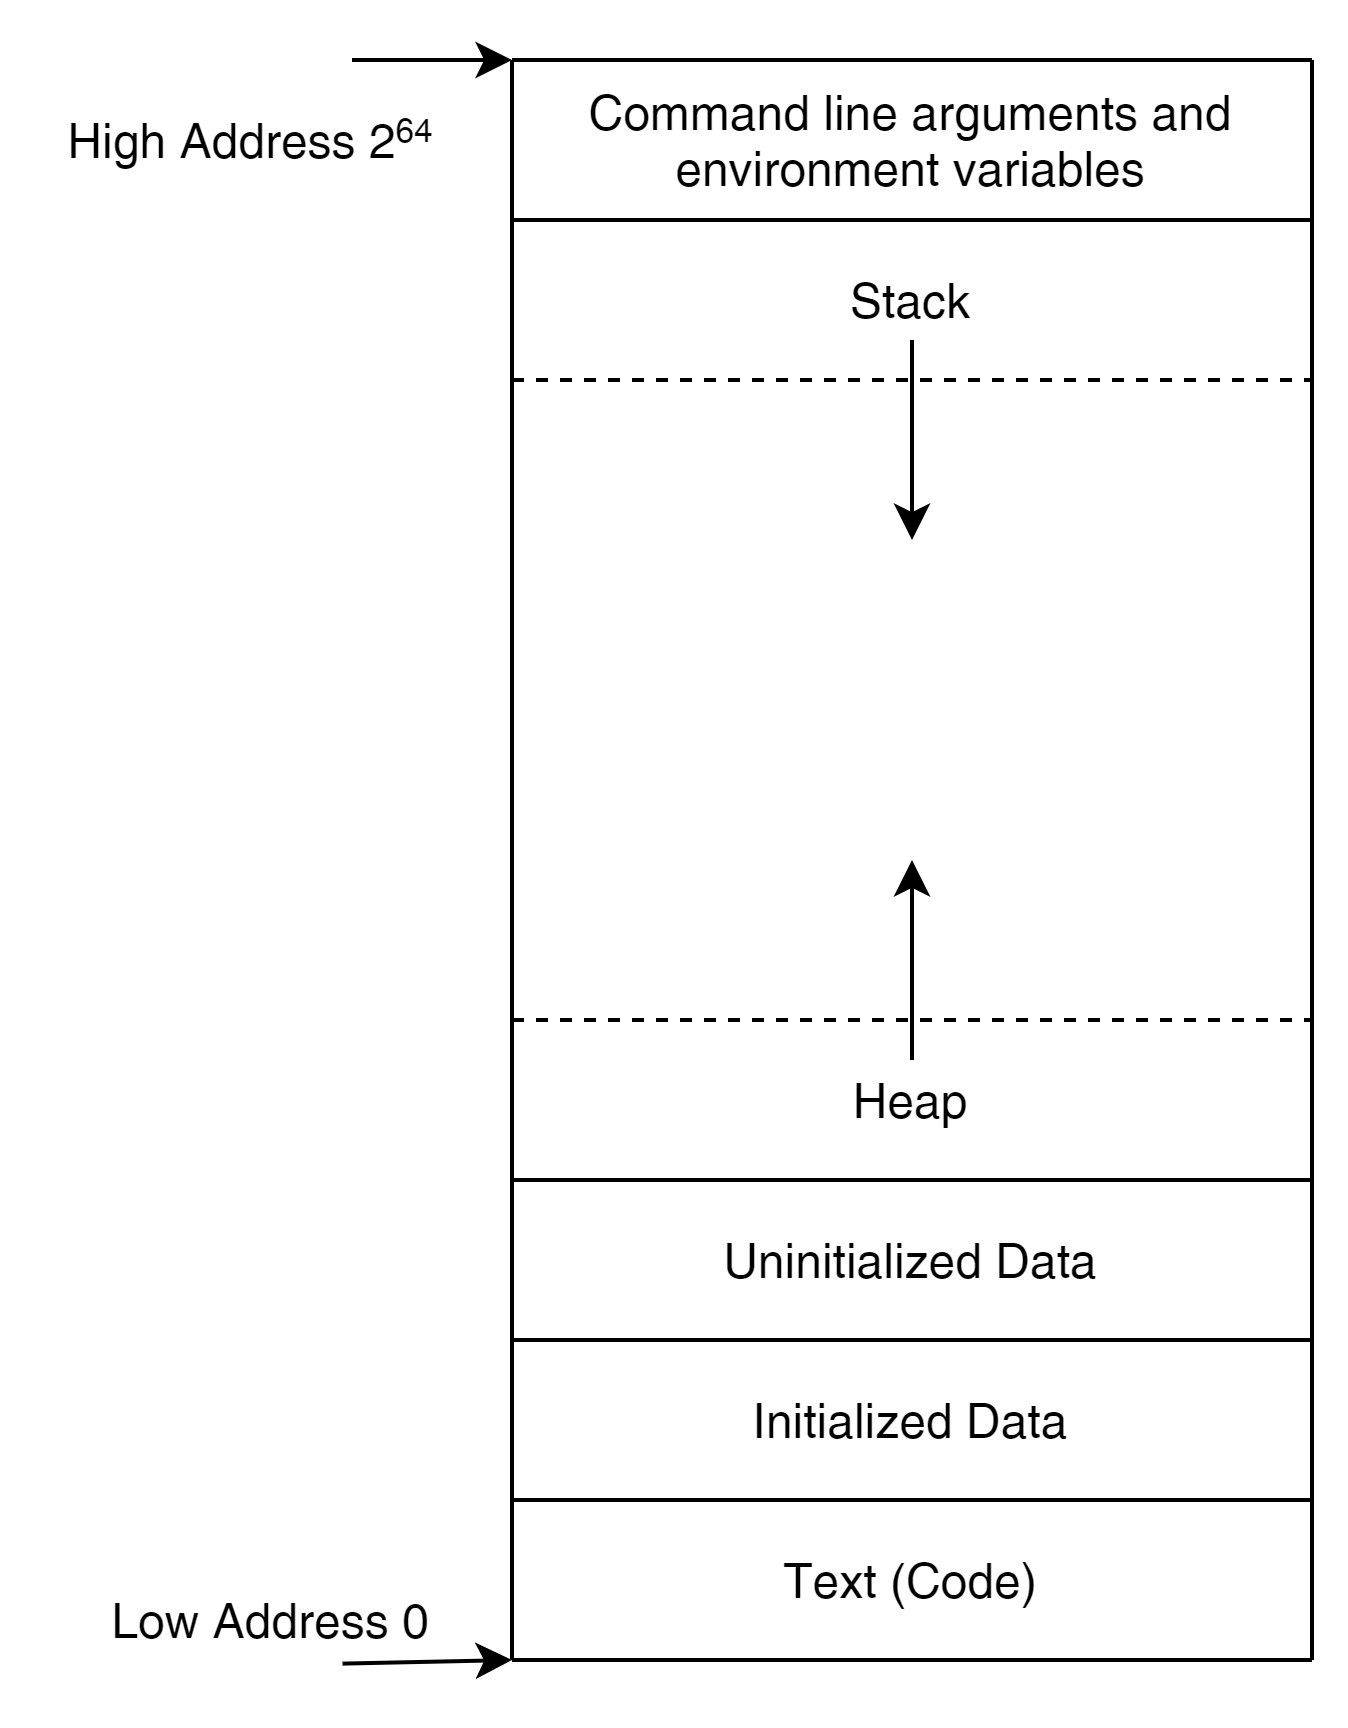
\includegraphics[height=0.4\textheight]{stack.png}
\end{center}
\end{multicols}

Accessing array and struct elements in C is done by calculating the offsets from the pointer to the base of the object to the element. For example, integers are \texttt{4} bytes, so accessing the \nth{10} element of an integer array would be done by calculating $\texttt{addr} + 10*4$.


\subsection{Problems with C Code}

Code written in C has a history of being \textit{very} bug prone\cite{common-bugs}. Due to the language's popularity and speed it is often used in security-critical applications. Many vulnerabilities that appear in C code are to do with incorrect memory management. The most common examples are dereferencing unknown memory locations, buffer overflows, accessing previously freed memory, reading uninitialized memory and double freeing a memory location.

The first example shows and example of an uninitialized pointer.

\begin{lstlisting}[language=C, caption=Dereference unknown memory location]
int main(){
    int *x;
    x[0] = 1;
    return 0;
}
\end{lstlisting}

\texttt{x} is uninitialized and points to a random place in memory, thus dereferencing \texttt{x} will result in undefined behaviour and most likely a segmentation fault.

The next example shows a classic buffer overflow, \texttt{strcpy} copies the memory at the location of the second argument to the location of the first argument until a null byte (\texttt{\char`\\x00}) is found in the input string.

\begin{lstlisting}[language=C, caption=Buffer overflow]
#include <string.h>
#include <stdlib.h>
int main(){
    char buf[4];
    char str[] = "Hello World!AAAAAAAAAAAAAAAAAAAAAAAAAAAAA";
    strcpy(buf, str);
    return 0;
}
\end{lstlisting}

Strings in C have a null byte at the end of string, which is called a \textit{null-terrminated string}. Thus the \texttt{strcpy} will attempt to copy the entirety of \texttt{str} into \texttt{buf}, overflowing \texttt{buf} and overwriting the memory addresses above \texttt{buf}. Because these variables are allocated onto the stack the overwritten memory could contain the current functions return address and allow control-flow hijacking by a malicious actor. This can lead to remote code execution on the target system.

The C11 standard defines five memory management functions\cite{iso_standard}, \texttt{aligned\_alloc}, \texttt{calloc}, \texttt{malloc}, \texttt{realloc} and \texttt{free}. The standard places a number of guarantees on the memory management.
\begin{itemize}
    \item Returned pointers are suitably aligned so that the space can be used for type casting.
    \item The lifetime of an allocated object is defined between the objects allocation and deallocation. The state of the object outside of these bounds is undefined.
    \item Each allocation will yield a pointer to an object disjoint from any other memory object.
    \item The returned pointer will point to the lowest address of the allocated memory.
    \item If the requested memory size is zero, then the behaviour is implementation specific and either a null pointer or the implementation will behave as if the size is non-zero with the catch that the resultant pointer is not used for memory access to an object.
\end{itemize}

Applying the guarantees to the example below shows how memory that has been freed or de-allocated can have unintended effects when accessed. 

\begin{lstlisting}[language=C, caption=Access previously freed memory, label={code:access_freed}]
#include <stdlib.h>
#include <stdio.h>
int main(){
    int *x;
    x = malloc(sizeof(int)*32);
    x[0] = 1;
    free(x);
    int *y = malloc(32*sizeof(int));
    y[0] = 2;
    printf("%d", x[0]);
    return 0;
}
\end{lstlisting}

There are no guarantees on the state of the region associated with \texttt{x} after the \texttt{free} call and thus any succeeding accesses to \texttt{x} are undefined. Then, when the object \texttt{y} is allocated, the object can be allocated to a non-disjoint region from the region for \texttt{x}. Thus, in some\footnote{depending on libc and operating system implementation} environments \texttt{y[0]=2} will override the value of \texttt{x[0]} and "2" will be printed.

The last class of undefined behaviour that shall be covered in this section is the double free. Double free's root cause is the same as Listing \ref{code:access_freed} with a different manifestation.

\begin{lstlisting}[language=C, caption=Double free, label={code:double-free}]
#include <stdlib.h>
#include <stdio.h>
int main(){
    int *x;
    x = malloc(4*sizeof(int));
    x[0] = 1;
    free(x);
    int *y = malloc(10*sizeof(int));
    y[0] = 2;
    free(x);
    return 0;
}
\end{lstlisting}

From the previous example it is possible for \texttt{x} and \texttt{y} to point to the same region of memory after the allocation of \texttt{y}, thus freeing \texttt{x} again will actually free a subregion \texttt{y} the size of the of \texttt{x}. In this case a region of size 4 at will be de-allocated.

\subsection{Detecting Undefined Behaviour in C Using Static Tools}
For performance and safety critical code, static analysis of code is the primary means of verifying the correctness and identifying undefined behaviour in a programs execution\cite{jourdan2015formally}.

The analysis for a given program is performed on the source code exclusively, and does not involve executing any part of the program. Various methods such as symbolic execution, model checking and data-flow analysis have achieved good accuracy at detecting undefined behaviour but due to the undecidability of the Halting problem there is no correct mechanical method for determining if a general program has undefined behaviour\footnote{There is a simple reduction from deciding whether a program will execute undefined behaviour to the Halting problem}.  

\subsection{Detecting Undefined Behaviour in C Using Dynamic Tools}
Dynamic analysis varies from static analysis by running the program on a real or virtual processor. Most dynamic analysis tools monitor the state of the program and track variable values and memory accesses for invalid operations. Depending on the type of analysis required different tools have different priorities. A security tool will "fuzz" the program and supply a large number of inputs to hunt down invalid operations while a performance tool will be more concerned with cpu time spent on functions and building a time based control-flow of the program. 

An example tool is Valgrind~\cite{seward2005using} which is an extensible framework for dynamic analysis and has inbuilt tools for memory debugging and detecting invalid malloc and free calls.

\section{Coq and Formal Verification}

\begin{quotation}
    \textit{`Coq is a formal proof management system. It provides a formal language to write mathematical definitions, executable algorithms and theorems together with an environment for semi-interactive development of machine-checked proofs.'}~\cite{coq_website}.
\end{quotation}

Whilst this project does not involve any writing of the Coq language there has been a large amount of \textit{reading} of Coq in this project due to CompCert being largely written in Coq. Coq has a large range of uses. For example, formally verifying that a compiler will produce a program that conforms to the specified execution even through optimizations (otherwise known as operational semantics) and formalizing and proving mathematical theorems. I will present an example from "A short introduction to Coq"\cite{introduction-to-coq} to show how a proposition for even and odd numbers would be written.

\begin{lstlisting}[language=Coq, caption=Coq definition of even and odd numbers]
Inductive even : N -> Prop :=
  | even_0 : even 0
  | even_S n : odd n -> even (n + 1)
  with odd : N -> Prop :=
  | odd_S n : even n -> odd (n + 1).
\end{lstlisting}

This is an example of a \textit{proposition} in Coq. Propositions are statements that can either be true or false. The other category of objects found in Coq are \textit{types}. Types are typically used for executable algorithms and mathematical definitions, whereas propositions are commonly used to define relations between states.

The Coq system has a functional programming language that supports these types and can be used to write programs. Furthermore, the programming language has an extraction feature\cite{coq-extraction} which allows Coq code to be extracted to certified and efficient functional programs. Coq currently has three output languages; OCaml\cite{leroy2014ocaml}, Haskell\cite{jones2003haskell} and Scheme\cite{dybvig2009scheme}. The CompCert compiler / interpreter that the project is using is extracted to OCaml and as such is the only extraction needed for the project. Coq can extract a series of Coq (\texttt{.v}) files to either a singular monolithic OCaml (\texttt{.ml}) file or separately extract each \texttt{.v} file to a corresponding \texttt{.ml} file\cite{coq_extraction}. The latter becomes much more appealing as the scale of the program grows and wrapper code can abstract out larger parts of the extracted program. The wrapper code is written in OCaml and can load any of the extracted OCaml modules. Once all OCaml code has been extracted / written all of the OCaml files can be compiled and linked to form an executable.

A number of the C semantics that I will be talking about further on in the project are propositions and defined as relations between states and can not be extracted out to OCaml.

\section{CompCert}\label{compcert}

\begin{quotation}
    \textit{
    `The CompCert project investigates the formal verification of realistic compilers usable for critical embedded software. Such verified compilers come with a mathematical, machine-checked proof that the generated executable code behaves exactly as prescribed by the semantics of the source program.'}~\cite{noauthor_compcert_nodate}
\end{quotation}
    CompCert's way of modelling memory is of key interest. The current version of CompCert models memory as a collection of \texttt{blocks}, each block modelling an area of memory in the program. The start and end points of each block are defined by  \texttt{low\_bound} and \texttt{high\_bound}, with pointers being represented by  $(b,i)$ pairs (the block identifier $b$ and an offset $i$). Pointer arithmetic is bounded by \texttt{low\_bound} and \texttt{high\_bound}. Attempting to access memory outwith the bound for a given block is an instance of \textit{undefined behaviour}. There are many other ways to encounter undefined behaviour (as defined in the C11 standard)\cite{iso_standard}.
    
    % The collection of blocks are contained in the \texttt{mem} type (with constant \texttt{empty : mem} denoting the empty state) and there are 7 operations that can be performed upon the memory:
    
    % \texttt{alloc, free, load, store, loadbytes, storebytes, drop\_perm}
    
    % the \texttt{drop\_perms} operation is special as it lowers the permission over a range of bytes. Details on permissions can be found in the relevant paper\cite{leroy2012compcert}.
    \begin{center}
        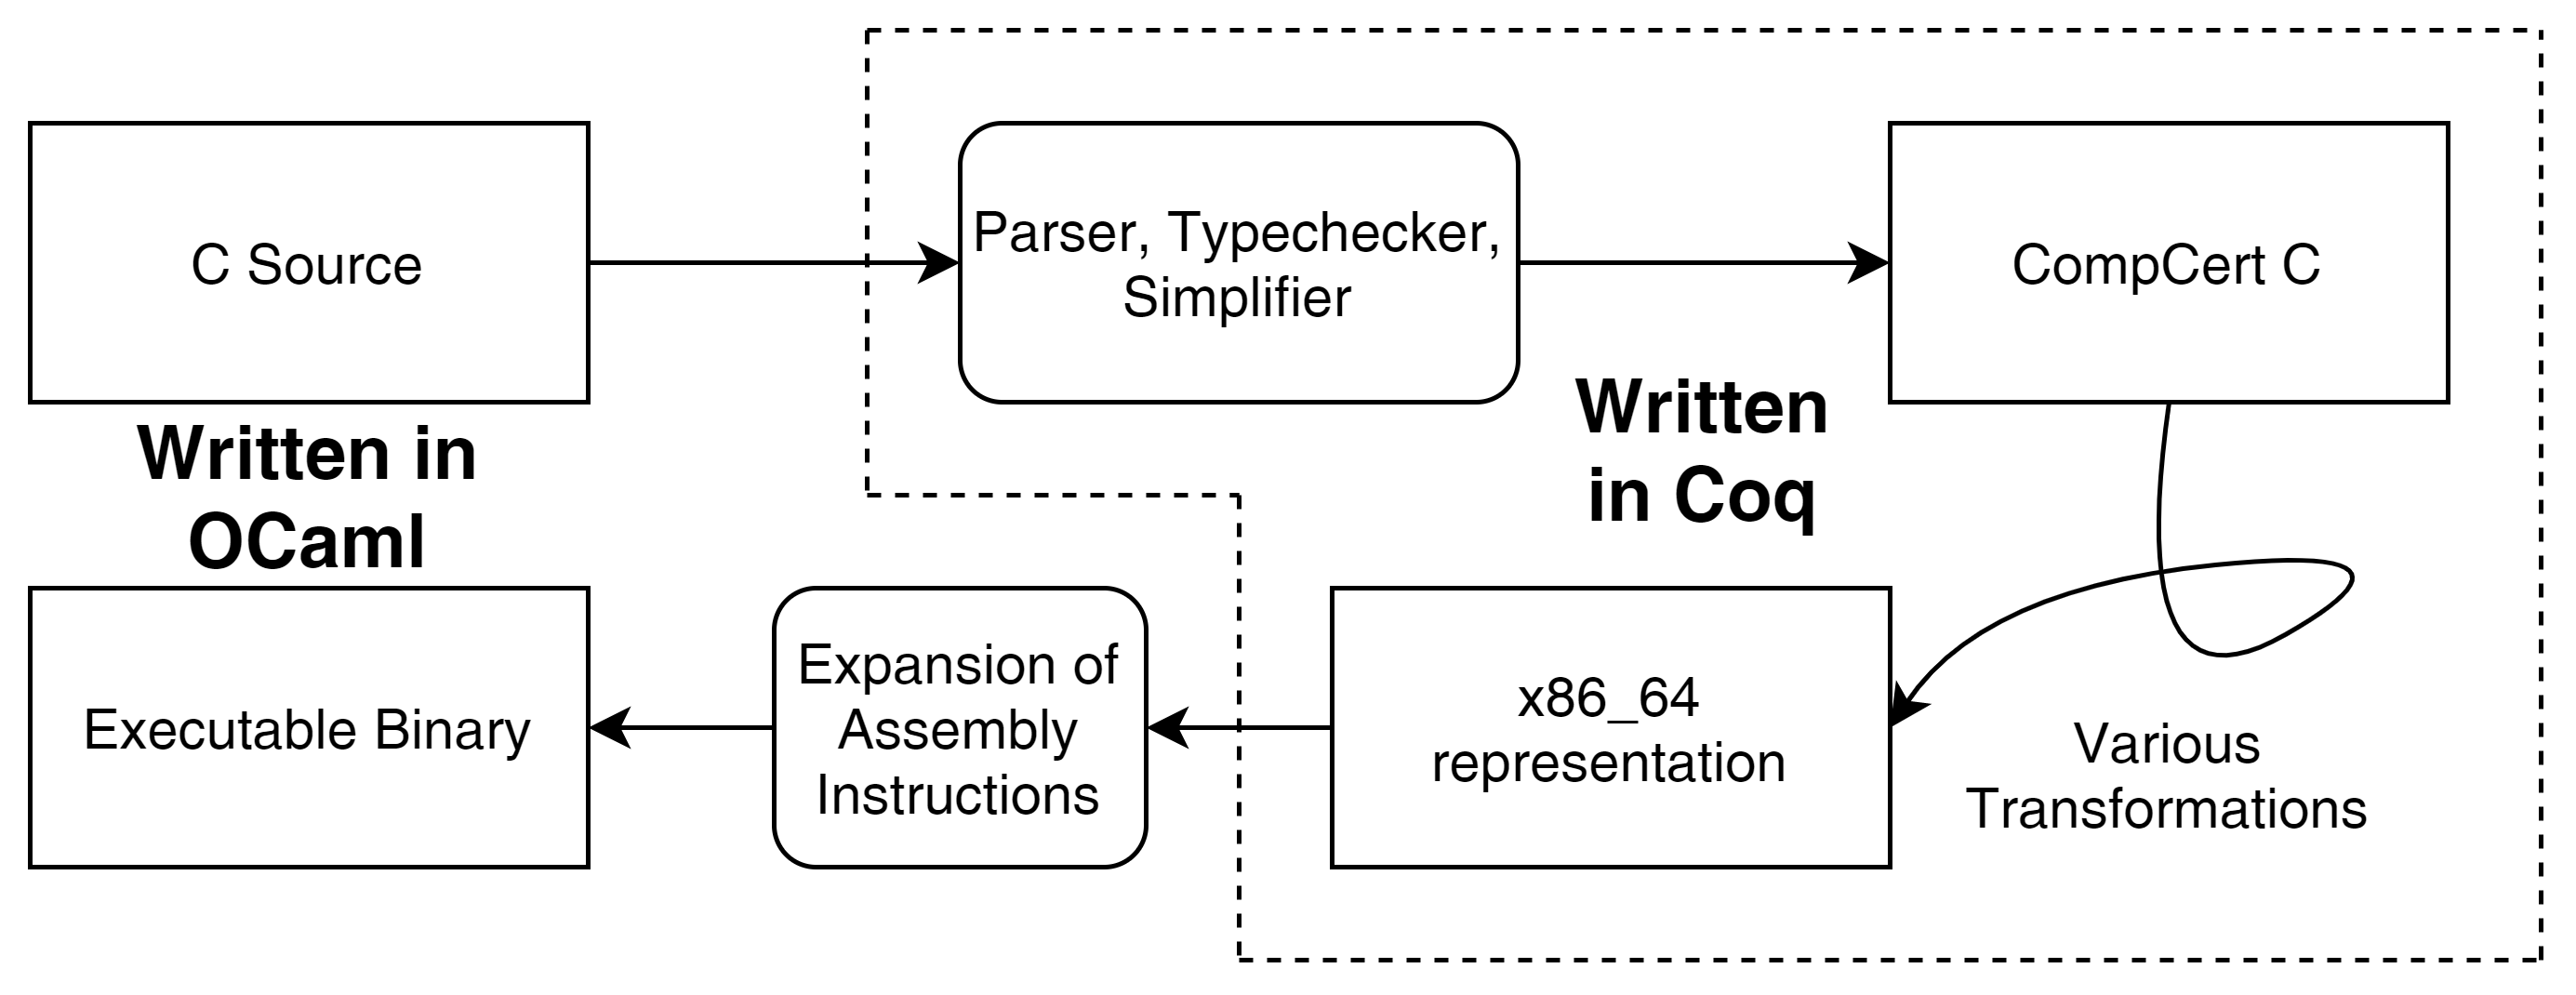
\includegraphics[width=0.8\textwidth]{ccomp-graph.png}
    \end{center}
    
    Instructions in CompCert are target platform specific and are defined in the respected target architecture's Coq Asm definition. For this project the x86\_64 architecture was chosen as the development machines are running on x86\_64 architecture and this will speed development time, there are also many tools available for x86\_64 due to it's abundance
    . The instructions build upon the abstract register types so that they can be reasoned about formally at compile time. Not all instructions are defined for the target architecture, and some operations are reduced into a simplified form (such as frame allocation). These reduced instructions are expanded when the program is emitted (interestingly, the expansion is not defined formally).
    
    Instruction execution is defined as operations over the register set, world state and memory state and is used in the compiler for verifying correctness over the compilation step.
    
    % The CompCert interpreter is given the program as . We can visualize CLight as a symbolization of the C source, such that every line of text, i.e. \texttt{int x = 1;} is represented more like $x : \texttt{int} \leftarrow 1$, a more abstract form. The interpreter then executes each line of code in a virtual model according to the C specification.
    
    % The CLight representation is where the compiler can perform static analysis, prove the correctness of a program and do model checking. These analysis's can be used by the interpreter as they are performed on the CLight representation without modifying it. 
    
    % This differs from the compilation step which introduces optimizations and produces a set of x86\_64 instructions that are emitted into a file.
    
% \section{Static Analysis of Source Code}\label{static-analysis-of-source-code}


% % \section{Dynamic Analysis}\label{dynamic-analysis}

\section{Disassembling}\label{disassembling}
In the context of this project disassembling refers to transforming machine code (i.e. bytes) into human-readable assembly. There are many existing tools with varying features sets that perform this task\cite{brumley2011bap, objdump, gdb} to varying degrees of complexity. Simple disassemblers are concerned with recreating the instructions while more complex programs attempt to reconstruct the control flow graph of the program and attempt to infer the semantics of the program.

For the purposes of this project we will only be concerned with object files, which have all of their function start addresses, function sizes and function names defined in the files symbol table.

The following diagram illustrates the compilation / disassembly process from a source file:

\begin{center}
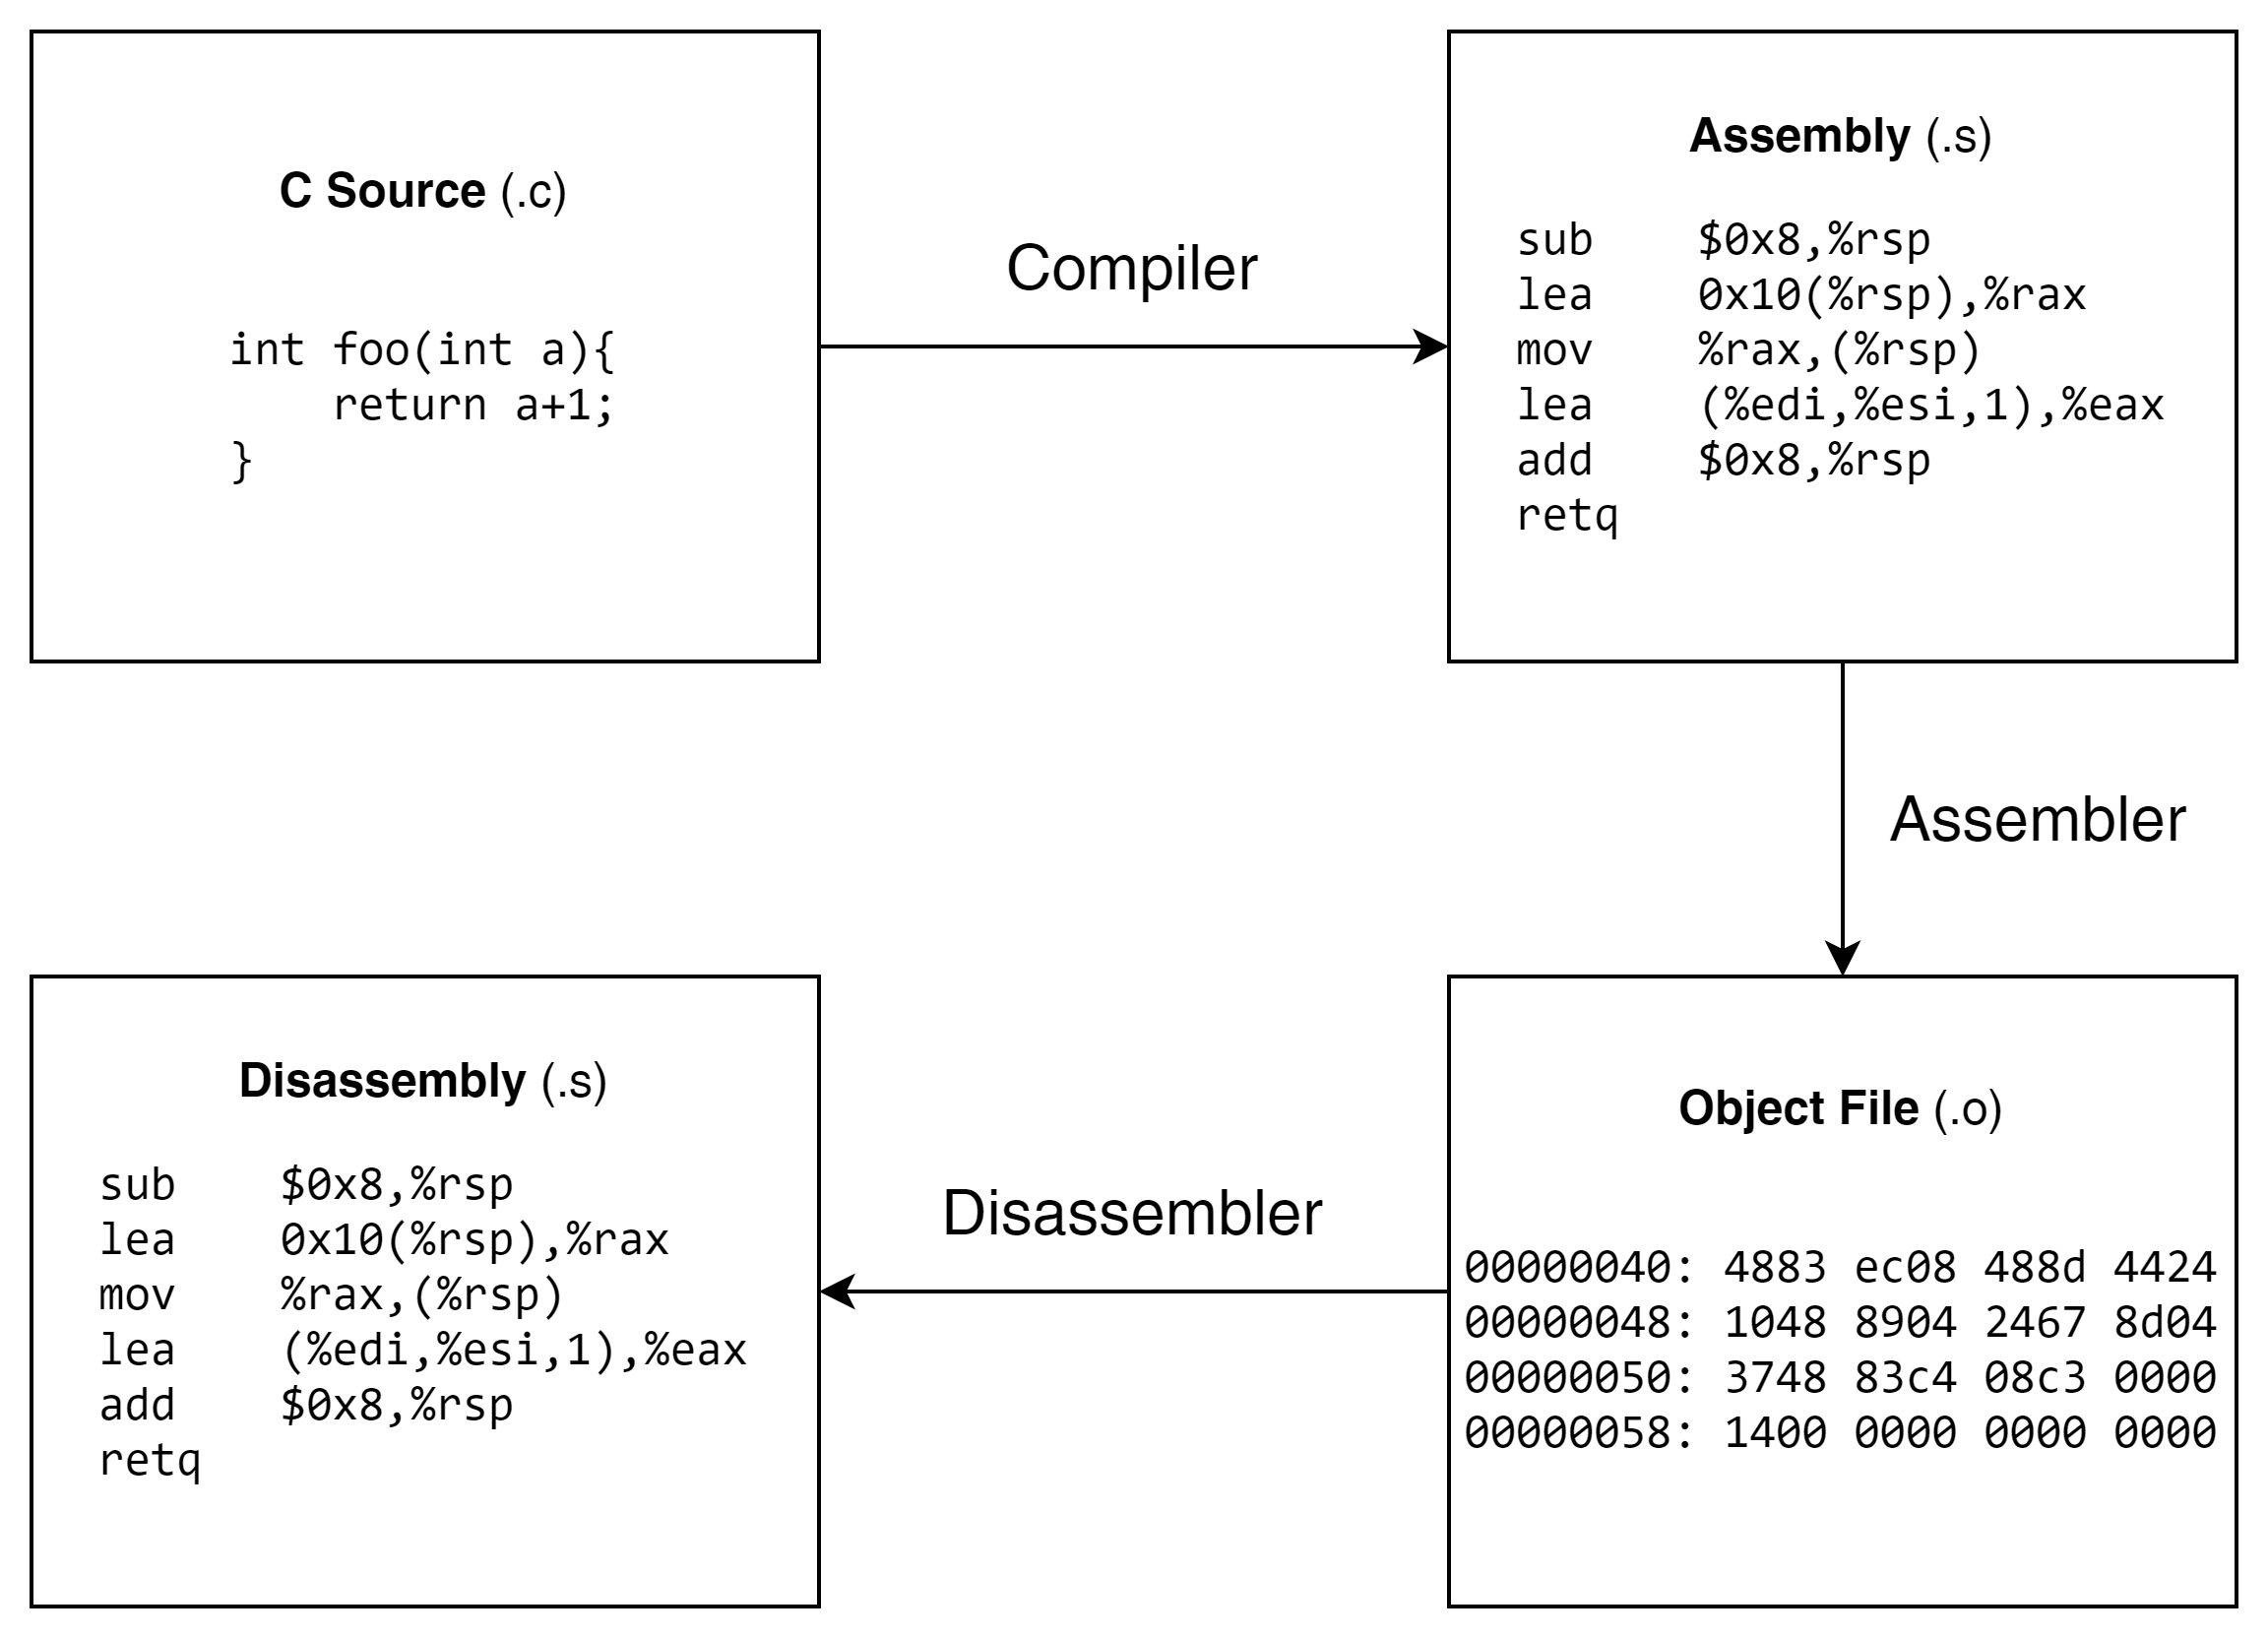
\includegraphics[width=0.75\textwidth]{disas.png}
\end{center}

% The process of disassembling a binary and correctly resolving function definitions is still unsolved and there are many literary works on the various attempts to push the frontier of disassembling accuracy. The industry standard for disassembling is IDA Pro alongside other disassemblers such as Binary Ninja, Radare2 and BAP. Most of these disassemblers implement variations of recursive descent and linear sweeping to reconstruct the control flow of the binary. Modern disassemblers have a 99\% accuracy at identifying function starts in the disassembly of non optimized binaries, but even the best performing disassemblers drop to 82\% identifying functions in aggressively compiler-optimized binaries\cite{andriesse2016depth}. 

\section{Binary Analysis Platform}\label{BAP}
The Carnegie Mellon University Binary Analysis Platform (CMU BAP)\cite{brumley2011bap} is a framework for performing analysis of compiled binary files. The framework comes with various utilities and libraries to analyse binaries, however the framework is mainly designed to be extensible with custom written plugins.

The BAP framework was initially chosen for the disassembly stage for two reasons. Firstly, BAP is written in OCaml and should therefore have a simple integration system with the CompCert project. Secondly, BAP has a system for performing \textit{passes} on assembly after it has been disassembled. This can be used for control flow reconstruction and reconstruction of the starts and relocations of heavily optimized functions. 

As the project developed, extracting the instruction specific mnemonics became an important task, and the BAP default output for instruction names and operands suited the needs of the project perfectly. A workaround to the integration issue was found by running BAP as a separate process and formatting the output of BAP to exactly match the required input to the project.

The BAP framework is designed for automated binary analysis and as such has large performance considerations making the framework an ideal candidate for use in this project. 

% The project is aiming to support object files (\textit{.o} files) for linking. These are similar to a compiled program; they contain compiled instructions, but they do not contain any executable code and haven't had any of the function calls linked. Object files very often (for the purposes of this project, always) contain relocation and linking information which is used to link the function calls inside the object file and linking calls in a compiled binary to the object's function. 


% \section{Expected Hurdles}
% The project has a few notable problems in implementing the project. Firstly CompCert is a massive project, and learning how the compiler is structured and finding where the code injection points should be will require a moderate understanding of how the Assembly and Interpreter are defined in CompCert. CompCert being large will also hinder integration with other OCaml libraries due to having to understand and edit custom makefiles for the project. 

% Calling functions from inside the assembly is another large area for issues to appear, as CompCert requires function calls to have a definition of the target function, and internal function calls inside the assembly will be unlikely to have the required information to correctly re-produce the details of the function call.


\chapter{Converting Object Files into CompCert Instructions}\label{Disassembling}

This chapter details the process of how I transformed compiled object files into the abstract instructions defined inside CompCert and how I used the operational semantics of instruction execution to build an assembly interpreter.

During this chapter, I will explain much of the process with reference to an example. The C source code for this example is as given.

\begin{lstlisting}[language=C, caption=example\_object.c, label=code:example]
#include <stdlib.h>
int bar(int n){
    int y = 0;
    int *x = malloc(n * sizeof(int));
    x[0] = 1;
    y = x[0];
    free(x);
    return y;
}
int foo(int a, int b){
    return bar(a) + b;
}
\end{lstlisting}

\section{CompCert Registers and Assembly Instructions}\label{compilers}
Registers and Assembly instructions are defined in CompCert by architecture specific abstract types. I decided on the x86\_64 architecture due to ease of testing, however, since the x86\_64 architecture has variable instruction length with a complex instruction set computer design and an emphasis on backwards compatibility formatting the instructions became significantly more complicated than if I had chosen a reduced instruction set architecture. An example of which is the \lstinline{load effective address} instruction, a complex add instruction for computing address offsets and is commonly used for simple addition. Each x86\_64 register in CompCert is defined uniquely and instructions are defined as composite types of registers, various types of values and address modes.

For example, the x86 integer registers are defined as:

\begin{lstlisting}[language=Coq]
Inductive ireg: Type :=
  | RAX | RBX | RCX | RDX | RSI | RDI | RBP | RSP
  | R8  | R9  | R10 | R11 | R12 | R13 | R14 | R15.
\end{lstlisting}

and the first couple of instructions as:

\begin{lstlisting}[language=Coq]
Inductive instruction: Type :=
  | Pmov_rr (rd: ireg) (r1: ireg) (** move contents of r1 to rd *)
  | Pmovl_ri (rd: ireg) (n: int)  (** move immediate n into rd *)
  | ...
\end{lstlisting}

Note how there are multiple CompCert instructions for each x86 instruction to handle the different mnemonics of each instruction, so CompCert treats them as different instructions. CompCert does not support every instruction defined in the x86\_64 specification, such as AAA - ASCII Adjust After Addition. Thus some object files will be incompatible with this project due to the unsupported instructions.

The function \lstinline{foo} in Listing \ref{code:example} is represented as this following set of CompCert instructions.

\begin{lstlisting}[language=C, caption=\lstinline{foo} from example]
int foo(int a, int b){
    return bar(a) + b;
}
\end{lstlisting}

\begin{lstlisting}[caption=CompCert instructions for \lstinline{foo}, label=code:instructions]
Pallocframe     24 16 0
Pmov_mr_a       RSP None 8 RBX
Pmov_rr         RBX RSI
Pcall_s         4
Pleal           RAX RAX RBX 1 0
Pmov_rm_a       RBX RSP None 8
Pfreeframe      24 16 0
Pret 
\end{lstlisting}
% \columnbreak
% \end{multicols}

With the assembly relating to the C code as follows:
\begin{enumerate}
    \item \lstinline{Pallocframe} allocates the stack frame for the function, this is found at the start of every function definition.
    \item \lstinline{Pmov_mr_a} stores the \lstinline{%RBX} register onto the stack to comply with the ABI. The ABI specifies that the \lstinline{%RBX} register is preserved across function calls, and thus because \lstinline{foo} makes use of \lstinline{%RBX} to store \lstinline{b} across the function call it places the current value of \lstinline{%RBX} onto the stack.
    \item \lstinline{Pmov_rr} moves the second argument \lstinline{b} of \lstinline{foo} into \lstinline{%RBX} so that it will be preserved across the function call.
    \item \lstinline{Pcall_s} performs a function call to the assembly located at function \texttt{4}. Which in this case is the function \lstinline{bar}. The passed arguments are \lstinline{%RDI} which contains the value of \lstinline{a}. 
    \item \lstinline{Pleal} adds the stored value \lstinline{b} in \lstinline{%RBX} to the function return value in \lstinline{%RAX}.
    \item \lstinline{Pmov_rm_a} restores the callers \lstinline{%RBX} value into the register from memory.
    \item \lstinline{Pfreeframe} de-allocates the stack frame which signals that the assembly has reached the end of the function.
    \item \lstinline{Pret} returns from this function to the current return address stored in \lstinline{%RA}.
\end{enumerate}

\section{Using objdump for Relocation Tables}\label{objdump}
objdump\cite{objdump} is a GNU binutils program for displaying various information about object files. The program is intended for assisting in work on compilation tools. 

The use of objdump in this project is to print the relocation entries of a compiled object file. Object files have not been linked to an executable and as such have not had any of the. There are three types of function calls that typically appear in an object file; calls to other functions inside the object file, calls to standard external functions like malloc or free and calls to external functions in other object files. The relocation table from the example is as follows:

\begin{lstlisting}
example_object.o:     file format elf64-x86-64

RELOCATION RECORDS FOR [.text]:
OFFSET           TYPE              VALUE 
000000000000001e R_X86_64_PC32     malloc-0x0000000000000004
000000000000002d R_X86_64_PC32     free-0x0000000000000004
0000000000000056 R_X86_64_PC32     bar-0x0000000000000004
\end{lstlisting}

I have written a Python script to match up the offsets to the instruction address in the object file and convert the function name (in this case foo, malloc and free) into the block numbers that the functions are located in (block construction and labelling is detailed in \ref{constructing-types}). To get the relocation information into our formatter Python runs objdump as a separate process using the subprocess module\cite{subprocess}.

objdump was chosen due to it's simple formatting, minimal setup and extensive documentation, alternatives include linuxs' \lstinline{readelf} program, but since objdump is feature complete for the needs of the project it was chosen as the relocation tool.

\section{Inclusion into CompCert}
While BAP offers an extension style model CompCert is a very large project with a non-trivial compilation procedure and integrating BAP into CompCert as a library was found to be too difficult to accomplish in the given time.  The build build system for CompCert is complex and ensuring that the 

The makefiles for the CompCert project are both lengthy and complicated and ensuring that the OCaml versions matched with BAP and various dependencies in opam was a lengthy process. 

Instead I decided to perform the disassembling step in a separate process before the execution of the interpreter. The instructions are printed from the Python process and loaded into CompCert using an \textit{in\_channel} in OCaml. Python was chosen as a wrapper for the disassembling step for three main reasons. Firstly, Python's syntax for string handling is concise and well suited to the transformations needed in the disassembling process. Secondly, Python is a scripting language and I wouldn't need to recompile the project every time I made a change to the wrapper as I would need to do if I wrote the formatter in OCaml inside CompCert. Finally, BAP comes with a wrapper for it's disassembly step in Python which produces a succinct description of each instruction. The BAP output in Python uses instruction names specific to the instructions' mnemonics. For example in x86\_64 the \lstinline{mov} instruction can accept registers, immediates or address modes for memory accesses as operands and instead of having to write a custom detector for the different mnemonics BAP outputs unique names for these different instructions. An example of the BAP python output in the form \lstinline{<instruction address> <instruction name> <list of operands>} is as follows:

\begin{lstlisting}[frame=lrbt, numbers=none]
0x40 SUB64ri8[Reg("RSP"), Reg("RSP"), Imm(0x18)]
0x44 LEA64r[Reg("RAX"), Reg("RSP"), Imm(0x1), Reg("Nil"), Imm(0x20), Reg("Nil")]
0x49 MOV64mr[Reg("RSP"), Imm(0x1), Reg("Nil"), Imm(0x0), Reg("Nil"), Reg("RAX")]
0x4d MOV64mr[Reg("RSP"), Imm(0x1), Reg("Nil"), Imm(0x8), Reg("Nil"), Reg("RBX")]
0x52 MOV64rr[Reg("RBX"), Reg("RSI")]
0x55 CALL64pcrel32[Imm(0x0)]
0x5a LEA64_32r[Reg("EAX"), Reg("EAX"), Imm(0x1), Reg("EBX"), Imm(0x0), Reg("Nil")]
0x5e MOV64rm[Reg("RBX"), Reg("RSP"), Imm(0x1), Reg("Nil"), Imm(0x8), Reg("Nil")]
0x63 ADD64ri8[Reg("RSP"), Reg("RSP"), Imm(0x18)]
0x67 RETQ[]
\end{lstlisting}

Comparing these instructions to the instructions in Listing \ref{code:instructions} there is a $1:1$\footnote{almost, there are a couple of exceptions, notably jump instructions.} mapping between the BAP instruction names and the CompCert instruction names.

To convert the BAP names for the mnemonic specific instructions to CompCert instructions I created a map of BAP instruction names to CompCert instruction names. I then wrote a Python function to match up the operands supplied by BAP with the required operands for the CompCert instructions and filter / swap the operands until they are in the correct order for CompCert.
 
I designed the output format from the wrapper as follows, with the top part of the following example being the format specification and the bottom part the foo function from before:



% I decided on an output format where each line starts with either an instruction name followed by space separated operands or a $>$ symbol followed by a function name. This design was led by ease of use in OCaml. Splitting the instruction names and operands is trivial with OCaml's string library and I can then match the instruction name to the assembly instruction type. Putting the function names at the end of the functions' assembly was so that I could build an arbitrary list of instructions and them on a $>$ match I can add the function to the global programs' functions and add a (\texttt{string * ident}) tuple to a list. This list is used when an external function is called to adjust the main function of the program to execute the external function.

% Here is the output format with an example.

\begin{lstlisting}[numbers=none,frame=lrtb,caption=Disassembly wrapper output format, label=format]
<instruction_name1> <register/value> <register/value> ...
<instruction_name2> <register/value> <register/value> ...
...
> <function_name1>
<instruction_name3> <register/value> <register/value> ...
<instruction_name4> <register/value> <register/value> ...
...
> <function_name2>

Pallocframe 24 16 0
Pmov_mr_a RSP None 8 RBX
Pmov_rr RBX RSI
Pcall_s 4
Pleal RAX RAX RBX 1 0
Pmov_rm_a RBX RSP None 8
Pfreeframe 24 16 0
Pret 
> foo
\end{lstlisting}

Note how closely the instruction names and formatting match the instructions in Listing \ref{code:instructions}. This is so that the amount of OCaml code to be written was minimal and was simple string matching. The only more complex case was memory addressing modes which has \textit{optional} parameters, thus I wrote an OCaml function to determine if the addressing mode was None (indicated by the respecitve register being "Nil").

Putting the function names at the end of each functions' assembly was so that arbitrary lists of instructions and then on a $>$ match the instructions can be turned into a function and then added to the global program. I also decided to add a (\texttt{string * ident}) tuple to a separate list with the functio name and the function location (an integer). This list is used when an external function is called to adjust the main function of the program to execute the external function.

\subsection{Resolving Relative Jumps}

Jump instructions proved to be a harder challenge than expected. Since instructions in CompCert do not have addresses relative jumps resulting locations are specified by \lstinline{Plabel} pseudo-instructions. Thus to correctly run the assembly the \lstinline{Plabel} instructions were required to be recreated in the correct positions and the jump operands updated with the correct \lstinline{Plabel} identifier. This was done by taking calculating the resultant address of the jump:

$$\text{Resulant address} = \text{Jump instruction address} + \text{offset}$$

and iterating through the functions instructions until a matching resultant address $\pm 1$ is found. My script then inserted a \lstinline{Plabel} with a unique positive identifier just after the resultant instruction and updated the jumps instructions operand with the new \lstinline{Plabel}'s identifier. Note that this approach will not directly match the original disassembly as I naively create \lstinline{Plabel} instructions for each jump instruction, and thus jump instructions that are intended to jump to the same place will now point to consecutive \lstinline{Plabel} instructions.

As I perform the manipulation of the instruction names I use the relocation information from objdump to fill in the information for internal calls. The Python-BAP module and objdump report different addresses for instructions so I subract \texttt{0xc0000040} from each address in the BAP instructions. BAP seems report all signed integers as unsigned so I added a conversion for instructions like relative jumps.

\subsection{Resugaring Frame Allocations}

Due to the way that CompCert handles memory blocks I recreate the frame allocation and frame destruction for function definitions by using the CompCert pseudo-instructions \texttt{Pallocframe} and \texttt{Pfreeframe} as seen in Listing \ref{format}. This is due to to the way CompCert creates blocks of memory in an abstract model rather than just adjusting the stack pointer (which is how assembly handles frame allocation). After examining the disassembled asm it became clear that there were three or five x86\_64 instructions at the start of the function allocating the frame and a single add instruction at the end of the function responsible for removing the function frame before the return instruction. To create the stack frame in CompCert I need to use CompCert's \texttt{Pallocframe} and \texttt{Pfreeframe} instructions which are unique to CompCert. 

To find the the values needed to reconstruct the frame management instructions I reversed the \texttt{Asmexpand.ml} file which handles the expansion of CompCert pseudo-instructions and built-ins to valid x86 instructions.

\begin{lstlisting}[language=OCaml, caption=Asmexpand.ml, firstnumber=496, framexleftmargin=14pt,]
let expand_instruction instr =
  match instr with
  | Pallocframe (sz, ofs_ra, ofs_link) ->
    if Archi.ptr64 then begin
      let (sz, save_regs) = sp_adjustment_64 sz in
      (* Allocate frame *)
      let sz' = Z.of_uint sz in
      emit (Psubq_ri (RSP, sz'));
      emit (Pcfi_adjust sz');
      if save_regs >= 0 then begin
        (* Save the registers *)
        emit (Pleaq (R10, linear_addr RSP (Z.of_uint save_regs)));
        emit (Pcall_s (intern_string "__compcert_va_saveregs",
                    {sig_args = []; sig_res = None; sig_cc = cc_default}))
      end;
      (* Stack chaining *)
      let fullsz = sz + 8 in
      let addr1 = linear_addr RSP (Z.of_uint fullsz) in
      let addr2 = linear_addr RSP ofs_link in
      emit (Pleaq (RAX, addr1));
      emit (Pmovq_mr (addr2, RAX));
      current_function_stacksize := Int64.of_int fullsz
    end else begin
      ...
    end
  | Pfreeframe (sz, ofs_ra, ofs_link) ->
    ...
  | ...
\end{lstlisting}

I've highlighted each \texttt{emit} call as this is where the frame allocation pseudo-instruction is converted into x86\_64 instructions. The first thing to note is that there are \textit{six} emit calls in this snippet compared to the three or five instructions I am expecting. This is because \texttt{cfi\_adjust} is a CFI profiling directive and not an actual instruction, note that the CFI directives have no effect on the generated assembly. This reduces us back to our three or five instructions. 

\begin{lstlisting}[language=x86-64]
sub    $0x8,%rsp
lea    0x10(%rsp),%rax
mov    %rax,(%rsp)
...    // Function instructions
add    $0x8,%rsp
...   // Either ret or function call
\end{lstlisting}

Reconstructing \texttt{Pallocframe} is relatively simple as CompCert inserts the frame allocation before any other instructions in a function. I can therefore extract the full size (\texttt{fullsz}) from the \texttt{lea} instruction which is either the \nth{2} or \nth{4} instruction depending on the number of saved registers and subtract 8 to get the size \texttt{sz}. I can get the \texttt{ofs\_link} from the addressing mode of the \texttt{mov} instruction.

Inferring the return address offset \texttt{ofs\_ra} is a more tricky task as the value of \texttt{ofs\_ra} is not emitted in the assembly and is used in the execution of \texttt{Pallocframe} in CompCert. Thus I have to rebuild the return address offset from the Coq semantics of the x86 stack layout.

\begin{lstlisting}[language=Coq, firstnumber=34, caption=Stacklayout.v]
Definition make_env (b: bounds) : frame_env :=
  let w := if Archi.ptr64 then 8 else 4 in
  ...
  let sz := oretaddr + w in (* total size *)
  {| fe_size := sz;
     fe_ofs_link := olink;
     fe_ofs_retaddr := oretaddr;
     ... |}.
\end{lstlisting}

On line \texttt{37} the stack size is set to the return address offset $+$ the wordsize (which is 8 for x86\_64). Thus the return address offset is calculate by
$$\texttt{ofs\_ra} = \texttt{sz} - 8.$$


% \begin{lstlisting}[language=Coq]
% Program Definition function_bounds := {|
%   used_callee_save := RegSet.elements record_regs_of_function;
%   bound_local := max_over_slots_of_funct local_slot;
%   bound_outgoing := Z.max (max_over_instrs outgoing_space) (max_over_slots_of_funct outgoing_slot);
%   bound_stack_data := Z.max f.(fn_stacksize) 0
% |}.
% \end{lstlisting}


% This is done by finding the offsets and sizes of the stack frames from the first three instructions in the function (which are responsible for allocating the stack frame) and omitting them from the instructions that are passed to the interpreter. 
\subsection{Constructing Correct Types in CompCert}\label{constructing-types}

Finally, I need to reconstruct the abstract type that CompCert executes, this type is the \texttt{program} type. The Coq definitions for the \texttt{program} type and other relevant types are given:

\begin{lstlisting}[language=Coq, caption =Asm.v program definition]
Definition code := list instruction.
Record function : Type := mkfunction { fn_sig: signature; fn_code: code }.
Definition fundef := AST.fundef function.
Definition program := AST.program fundef unit.
\end{lstlisting}

with \texttt{AST.program} and \texttt{AST.fundef} defined in the AST.v file as follows.

% (** Whole programs consist of:
% - a collection of global definitions (name and description);
% - a set of public names (the names that are visible outside
%   this compilation unit);
% - the name of the ``main'' function that serves as entry point in the program.

% A global definition is either a global function or a global variable.
% The type of function descriptions and that of additional information
% for variables vary among the various intermediate languages and are
% taken as parameters to the [program] type.  The other parts of whole
% programs are common to all languages. *)
% Inductive globdef (F V: Type) : Type :=
%   | Gfun (f: F)
%   | Gvar (v: globvar V).

\begin{lstlisting}[language=Coq, caption = AST.v program record definition and fundef definition]
Record program (F V: Type) : Type := mkprogram {
  prog_defs: list (ident * globdef F V);
  prog_public: list ident;
  prog_main: ident
}.

...

(** Function definitions are the union of internal and external functions. *)
Inductive fundef (F: Type): Type :=
  | Internal: F -> fundef F
  | External: external_function -> fundef F.
\end{lstlisting}

So,

\begin{itemize}
    \item The \texttt{code} type is a list of instructions
    \item The \texttt{function} record is a tuple of function signatures and corresponding function code.
    \item \texttt{fundef} are the union of Internal and External functions. They represent whether a function is defined inside the program or whether the function is defined in an external file.
    \item The \texttt{program} definition is a 3-tuple containing 
    \begin{itemize}
        \item A list of functions and their \texttt{ident} (location) in the code. The locations are arbitrary positive integers requiring successive pieces of code be successively numbered.
        \item A list of \texttt{ident} corresponding to each public function.
        \item An \texttt{ident} defining the entry point of the program.
    \end{itemize}
\end{itemize}

For a significant portion of the projects duration I made an assumption that the function signature was required either in the global environment construction or when calling internal functions. Reconstructing the functions proved to be non-trivial. I spent a long time theorizing ways to reconstruct the function signatures perfectly. I will detail the methods I could have taken to reconstruct the function definitions in the case that these methods would have been required.

\begin{enumerate}
    \item Construct the program every time a function is called with the called function as the "main" function,  and no other functions in the program, this way I can ensure that the function contains the function signature.
    \item Since the external functions will be called from inside the interpreter I can assume that the called function will have the same function definition as the caller, therefore I can reconstruct each function signature from the signatures in the CompCert C interpreter program before the interpreter is started but after the C source file is processed.
    \item I can require that object files contain a corresponding header file that contains the function signatures for every function in the object file. Then it is a simple matter of matching up the header file call signatures with the disassembly functions. This appraoch would again happen before the interpreter is started.
    % \item Construct the AST once with the first function as the main function and adjust the program counter with respect to the called function.
\end{enumerate}
Of these three methods, I was most keen on the third as the approach does not reduce the functionality of the object file. The other two approaches would not be able to call internal functions inside the object file which would severely limit the possible programs that could be written.

However, it turns out, after a deep analysis of how the global environment is set up and how call instructions and jump instructions are executed I don't need the correct function signatures at all! I can in fact just construct dummy signatures and disregard ever needing them again.

I believe this is because CompCert constructs the function definitions in the assembly program to be able to prove the transformation from CompCert C into assembly is correct. Understanding the exact reasons for this are out of the scope of this project.

\subsection{Internal Function Calls and Function Numbering}
\begin{verbatim}
    # todo
\end{verbatim}

\subsection{External Function Calls}

The last part of the program construction that I needed to deal with were the external calls from inside the object file to outside the object file. I have not implemented the general case due to time limitations, but it should be possible to do this as  an extension of this work.

To extend the implementation to the general case the interpreter would need to be able to take multiple object files as arguments. Separate programs would need to be constructed for each object file while resolving all of the relocations of the external calls. This should be doable by carefully setting up the locations (\texttt{ident}) of the functions and ensuring that the relocations point to the correct block in the program that the called function is in.

For this project I have hard coded in a small number of external functions to the start of the program so that I could test the detecting of undefined behaviour for memory allocations. I did this by placing \texttt{malloc} and \texttt{free} in blocks 1 and 2 of the program respectively. Instead of using assembly instructions for \texttt{malloc} and \texttt{free} I call the implementation of \texttt{malloc} and \texttt{free} defined Cexec.v that is extracted to OCaml.


\chapter{Extensions to the CompCert Interpreter}\label{ccomp}
In this chapter I will present the steps I took to implement my aims into the CompCert interpreter and any design decisions I took in the process. 

To aid in the understanding of the data flow of the project, the following flow chart shows how C source files are transformed into the executable environment that I have set up. I will first detail how I enabled the execution of instructions before moving onto how the interpreter interacts with the execution.

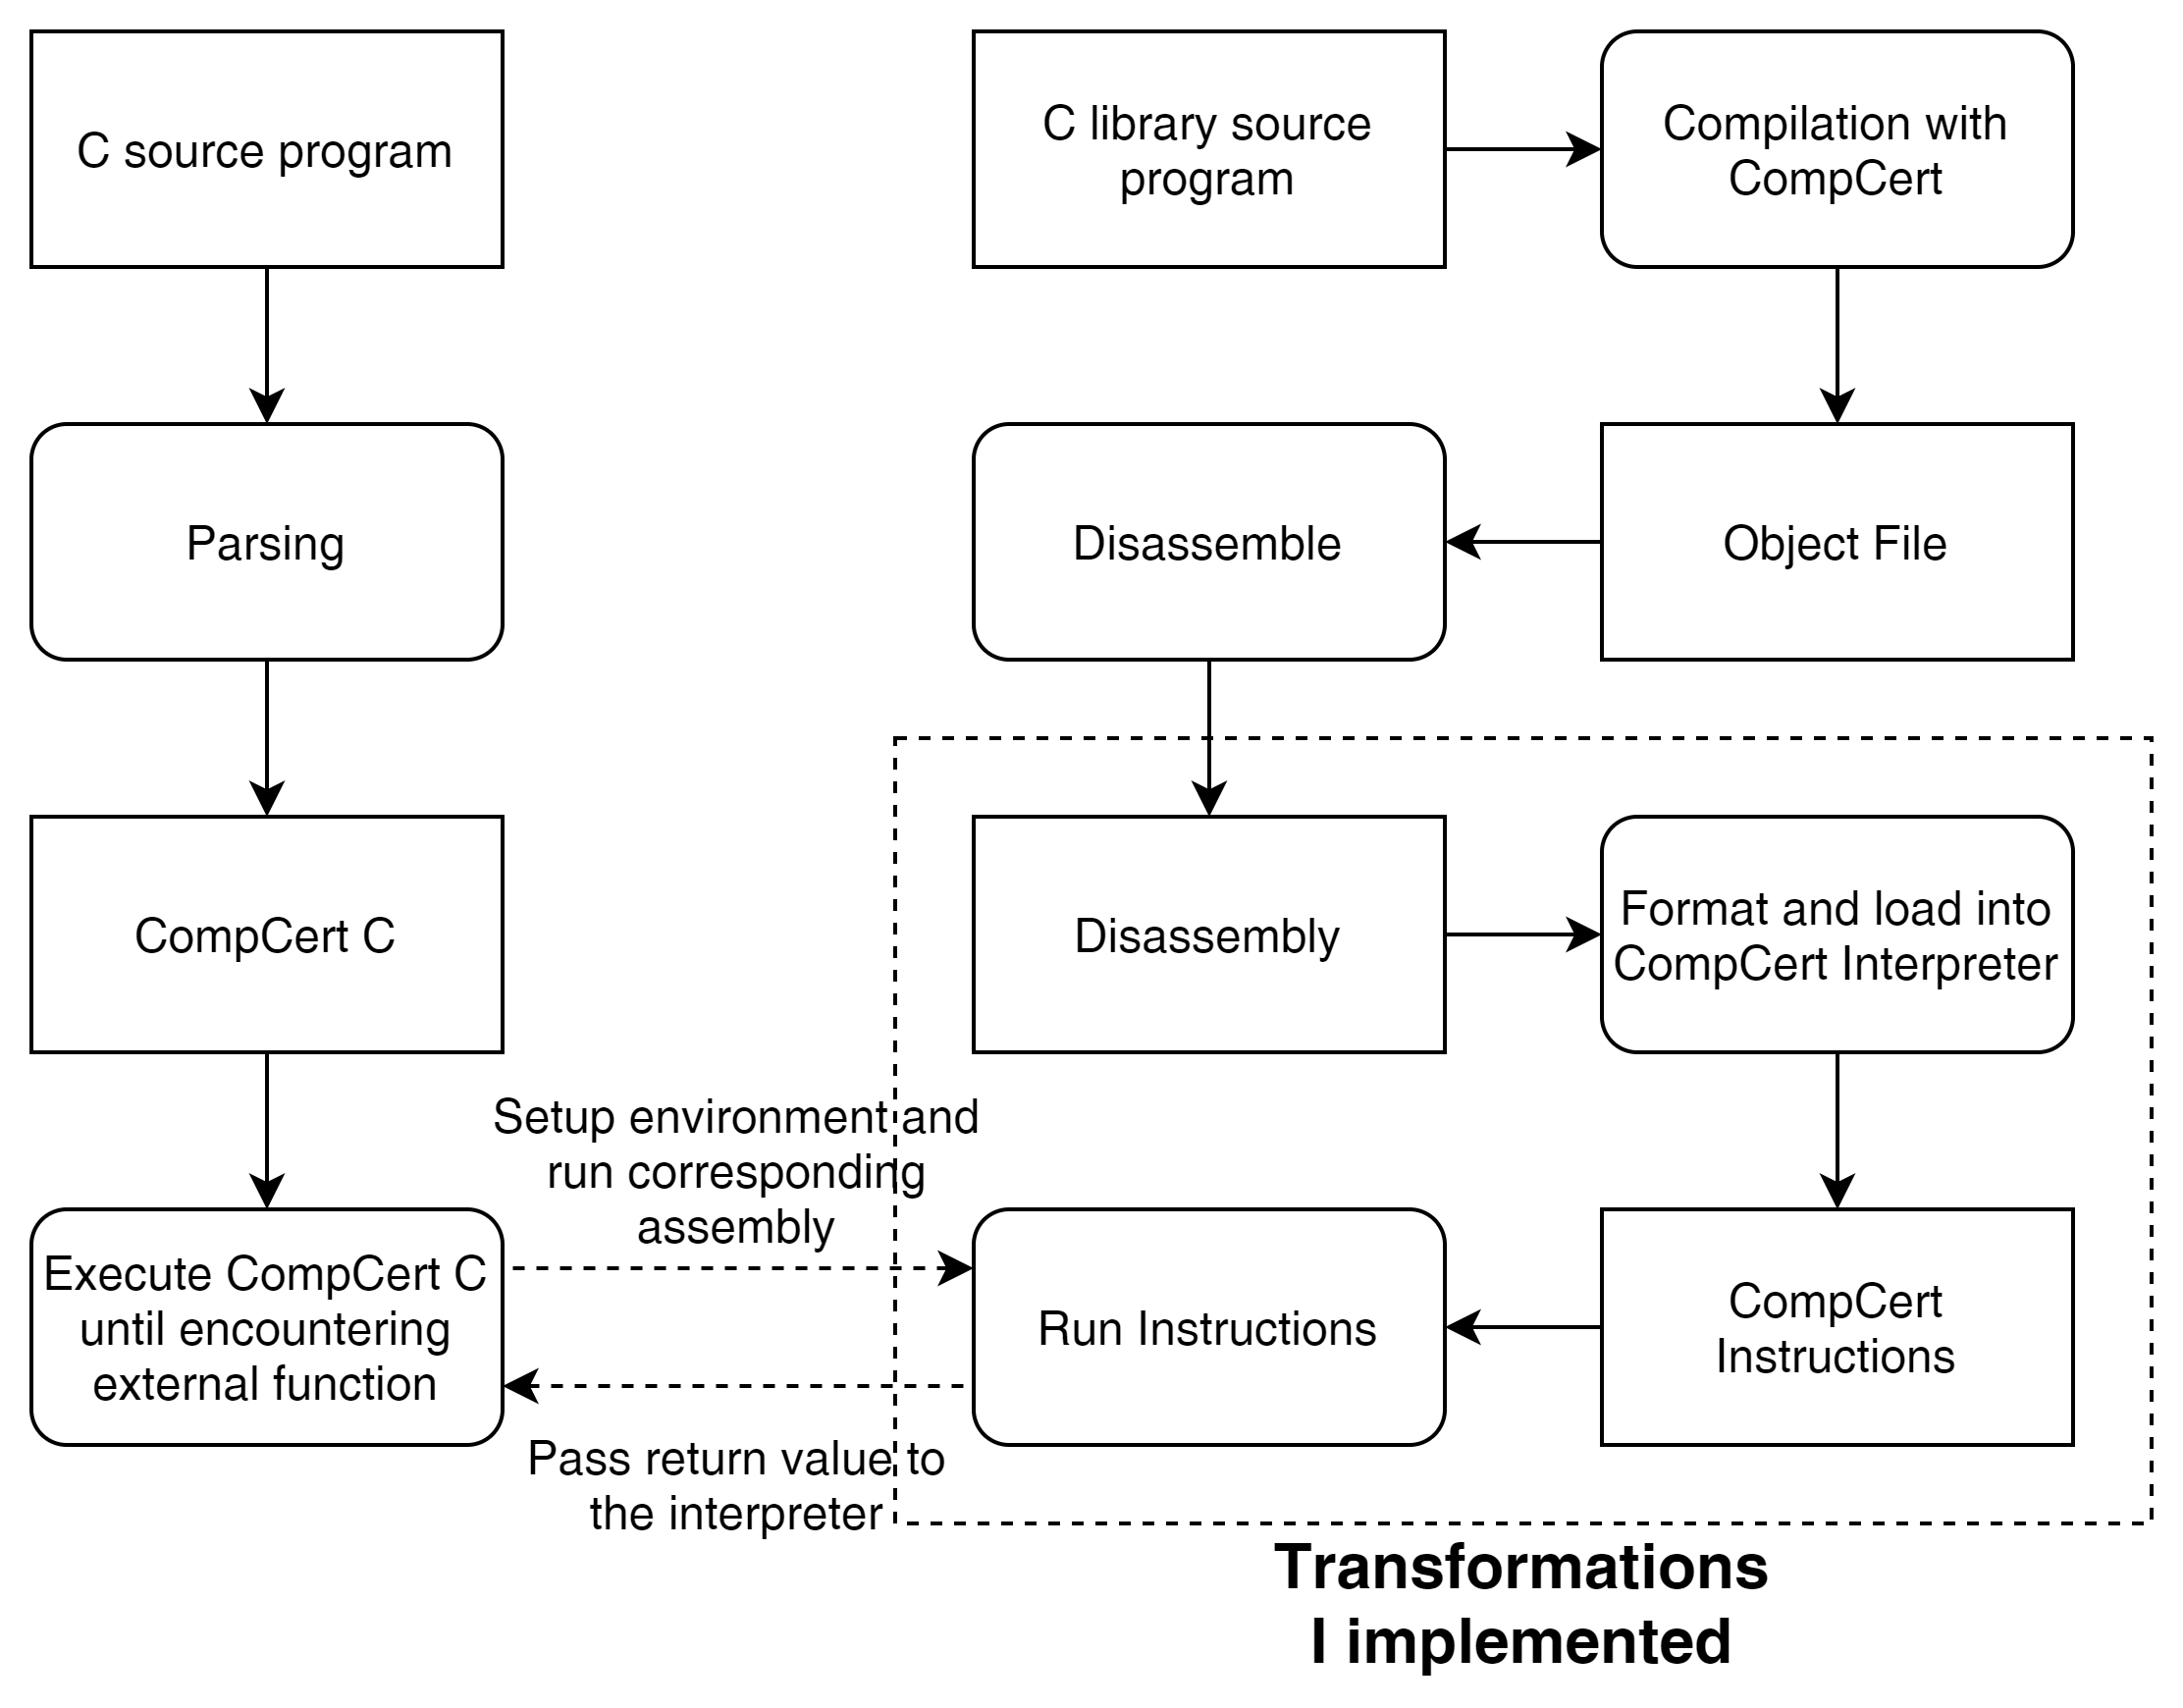
\includegraphics[width=\textwidth]{data_flow.png}

\section{Instruction Execution}\label{execution}
Execution of instructions is defined in the \texttt{Asm} Coq file, this is needed for CompCert's model to verify that the execution of the program defined by the C specifications matches the execution of the machine instructions after optimizations. Since the compiler needs to describe execution the \texttt{Asm} file contains a description of instruction execution:

\begin{lstlisting}[language=Coq]
Inductive step: state -> trace -> state -> Prop :=
  | exec_step_internal:
  forall b ofs f i rs m rs' m',
  rs PC = Vptr b ofs ->
  Genv.find_funct_ptr ge b = Some (Internal f) ->
  find_instr (Ptrofs.unsigned ofs) f.(fn_code) = Some i ->
  exec_instr f i rs m = Next rs' m' ->
  step (State rs m) E0 (State rs' m')
  | exec_step_builtin:
    ...
  | exec_step_external:
    ...
\end{lstlisting}

Where \texttt{b} is the block of instructions, \texttt{ofs} is the offset from the start of the block, \texttt{f} is the current function containing the instruction, \texttt{i} is the instruction, \texttt{rs} is the set of registers, \texttt{m} is the memory state and \texttt{rs'} and \texttt{m'} are the next step of \texttt{rs} and \texttt{m} after instruction execution.

On line 4 the block and offset are set\footnote{Set is a slight misnomer, in coq each line is defining a relation between the left and right hand side} from the program counter. The block is then used to get the current function \texttt{f} in line 5. Line 6 finds the instruction to execute from the functions code and the offset. The instruction can then be executed on the register set and memory giving the resultant register set and memory on line 7. Finally the step is defined inductively between states on the \texttt{rs'} and \texttt{m'}.

I have extracted this manually into an OCaml implementation as Inductive propositions cannot be extracted out by the machine. 

The \texttt{Asm} Coq file also defines the semantics of entire program execution which I can use to execute library functions by adjusting the initial program counter to the start address of the called library function:

\begin{lstlisting}[language=Coq]
Definition semantics (p: program) :=
  Semantics step (initial_state p) final_state (Genv.globalenv p).
\end{lstlisting}

I construct our initial state slightly different from the given \texttt{Asm} implementation. I initialize an empty memory state and set every register (including the return address (RA) and stack pointer (SP) to \texttt{Nullptr}. The program counter can be set manually or by calling the global environments' symbol address resolution function on the location of where execution should start. I chose the latter for ease of use and give the address resolution the value for the function location like so

\begin{lstlisting}[language=Ocaml, numbers=none]
let pc_init = Genv.symbol_address fge local_asm.prog_main Ptrofs.zero
\end{lstlisting}

% The second option was chosen so that I can call internal functions inside the library. Each function in the CompCert program has a unique value and I can keep a mapping of \textit{function name} $\rightarrow$ \textit{function code}. The drawback of choosing this method is that I would need to create function signatures for each internal function to 
% correctly recreate the call instructions. However, since the function signatures aren't actually used in the execution of call instructions I can disregard the calling convention and construct a dummy signature for the call.\footnote{Unfortunately for the project, it took me \textit{far, far, far} too long to realise this.}

% % For the purposes of this project we can assume that the linked file has a corresponding header file containing all internal function signatures, which we can then extract from the header file and use to build our CompCert program.

% After I have built a valid CompCert program I can create a global environment from the program which contains information about the programs functions and is required for many functions available in CompCert.

The last part I need for program execution is to implement a definition of a final state. In the initial state I set the RA to a \texttt{Nullptr} and so I can just add a check for the program counter being a \texttt{Nullptr} into my implementation of the instruction execution.

\section{Interpreter}
The CompCert interpreter is built upon the C semantics that the CompCert compiler is built upon, therefore any behaviour that is undefined for a given program in CompCert C will manifest in that programs' execution in both the compiled program and the interpreter. When a compiled program encounters undefined behaviour it will either crash or continue to execute after the undefined behaviour leading to outcomes that the programmer may have not intended. In contrast, the interpreter will halt execution when undefined behaviour is encountered and report the issue. 

The interpreter is by default limited to just six external functions~\cite{interpreter-manual} which are implemented within the interpreter:
\begin{verbatim}
    printf                __builtin_annot
    malloc                __builtin_annot_intval
    free                  __builtin_fabs
\end{verbatim}

So to get any useful functionality out of the interpreter it needs support for maths libraries, I.O. operations and a large chunk of the C standard library.

\section{Extending the CompCert Interpreter}\label{extending}
I extend the point at which the CompCert interpreter calls external functions, namely\newline \lstinline{do_external_function}. The function as given only has a hard coded implementation for \texttt{printf}, I have extended this by matching on an arbitrary string\footnote{I've left the \texttt{printf} case handling in so that \texttt{printf} will work without linking stdio} and finding the called function's name in the CompCert program. I can then set up the initial state as defined in \ref{execution}. After setting up the state I can make adjustments to the register set and the memory state to insert the function arguments either into the registers or onto the stack. The locations of the arguments can be inferred from the called functions' signature (which is given in the corresponding header file for the library). I am using the calling conventions for x86\_64 as defined in the \texttt{Asm} Coq file which is the System V AMD64 ABI calling convention common on Linux and OS X 64 bit systems. This calling convention will not be compatible with binaries compiled with different calling conventions without having knowledge of the binary's calling convention and having calling convention specific function to put the arguments in the correct places. A notable feature of the ABI is that the stack is 16 byte aligned rather than the a word aligned\footnote{This caused a large source of confusion in testing that should have been spotted sooner, but hey, I know lots about calling conventions now!}.

% After I finish executing the desired external function, I extract the resultant value from the \texttt{RAX} register and return the value to the interpreter which can continue execution. I currently do not support returning pointers from external objects as this would require copying the region of memory where the pointers' object resides into the interpreters memory state and adjusting the pointer to point to the new correct place. This would require a reasonable amount of work and would not handle the general case where a pointer may point to another pointer and so forth. At that point it may be worth using the interpreters memory state for the called function and ensuring that the called function doesn't attempt to make any changes to interpreter memory that is already set.  
\chapter{Evaluation}\label{eval}

The evaluation of the extended interpreter was carried out in two stages. The first stage evaluated the interpreter against custom written object files, designed to be small and test specific, known parts of the interpreter. The second stage was focused on real world object files. Due to time constraints the implementation is not able to handle some more complex test cases, in which case we will describe modifications and extensions to the implementation that would allow the examples to work with the project.

\section{Evaluation of Custom Object Files}

All of the object files were compiled with CompCert so that there were no unsupported instructions in the generated object file. The object files were written in an incremental fashion, with the easiest to implement features tested first and the more complex parts of the project evaluated later.

I will provide a series of examples showing the intended functionality of the project. The amount of detail in each example decreases to keep the explanations short and to the point, the full file contents and debug information can be found in the Appendix.

\subsection{Integer Arguments}

Integer arguments are the most basic feature that verifies a working minimal implementation. Here is an example source file which calls a trivial add function in an object file.
\begin{multicols}{2}
\begin{minipage}{0.5\textwidth}
\begin{lstlisting}[language=C, caption =call\_add.c]
int add(int a, int b);
int main(){
    int x = add(2,4);
    printf("x: %d\n",x);
    return 0;     
}
\end{lstlisting}
\end{minipage}
\begin{lstlisting}[language=C, caption=add.c]
int add(int a, int b){
    return a+b;
}
\end{lstlisting}
\end{multicols}

After compiling \texttt{add.c} into an object file with \lstinline{ccomp add.c -c -o add.o} we can disassemble the object files' text section to view the instructions relating to \lstinline{add(int a, int b)}.


\begin{multicols}{2}
\begin{minipage}{0.5\textwidth}
\begin{lstlisting}[language=x86-64, caption=add.o disassembly]
sub    $0x8,%rsp
lea    0x10(%rsp),%rax
mov    %rax,(%rsp)
lea    (%edi,%esi,1),%eax
add    $0x8,%rsp
retq   
\end{lstlisting}
\end{minipage}
\begin{lstlisting}[caption=Output of disassembly wrapper]
Pallocframe 16 0 0
Pleal RAX RDI RSI 1 0
Pfreeframe 16 0 0
Pret
> add
\end{lstlisting}
\end{multicols}

After resugaring there are 4 instructions in the output, the 2 instructions for frame allocation and de-allocation, the load effective address instruction which is a complex x86 instruction with that is commonly used for simple addition and the return instruction. Even though there are no local variables declared on the stack the frame allocations still take place.

Running these files in our project produces the following debug output showing the instruction execution.

\begin{lstlisting}[frame=lrtb, numbers=none, caption=\texttt{\$ ccomp -interp add.c -link add.o}]
Pallocframe
Pleal
Pfreeframe
Pret
x: 6
Time 19: observable event: extcall printf(& __stringlit_1, 6) -> 1
Time 24: program terminated (exit code = 0)
\end{lstlisting}

The number 6 is printed to \lstinline{stdout} and thus this is a demonstration of a working implementation.

\subsection{Mixed and Arbitrary Length Arguments}
This example demonstrates how the external functions can accept both integer and floating point arguments and correctly places them in the respective registers according to the ABI.

\begin{lstlisting}[language=C, caption=call\_mixed.c]
#include <stdio.h>
float multiply(int a, float b, int c, int d, float e);
int main(){
    printf("%f\n", multiply(2, 3.f ,1 ,2 ,5.f));
    return 0;
}
\end{lstlisting}

\begin{lstlisting}[language=C, caption=mixed.c]
float multiply(int a, float b, int c, int d, float e){
    return a * b * c * d * e;
}
\end{lstlisting}

The ABI convention fills up the integer registers and floating point registers first before placing arguments on the stack. I have not added support for arguments on the stack due to time limitations. This is due to the uncertainty in how CompCert lays out the memory and initializes the stack pointer when setting up the assembler global environment. This would require time spent researching the CompCert implementation of stack arguments.

\begin{lstlisting}[frame=lrtb, numbers=none, caption =\texttt{\$ ccomp -interp call\_mixed.c -link mixed.o}]
60.000000
Time 11: observable event: extcall printf(& __stringlit_1, 60.) -> 10
Time 16: program terminated (exit code = 0)
\end{lstlisting}

\subsection{Calling Internal Functions}

Calling internal functions is a necessity for a large amount of functionality in C. This example demonstrates this projects' ability to do so.

\begin{multicols}{2}
\begin{lstlisting}[language=C]
#include <stdio.h>
int bar(int a);
int main(){
    printf("%d\n", bar(4));
    return 0;
}
\end{lstlisting}

\begin{lstlisting}[language=C]
int foo(int a){
    return a+1;
}

int bar(int a){
    return a + foo(a);
}
\end{lstlisting}
\end{multicols}

\begin{lstlisting}[frame=lrbt, numbers=none, caption=\texttt{\$ ccomp -interp call\_malloc\_free.c -link malloc\_free.o}]
9
Time 11: observable event: extcall printf(& __stringlit_1, 9) -> 2
Time 16: program terminated (exit code = 0)
\end{lstlisting}

And as is show by the terminal output $4+(4+1)=9$ is printed, with more detailed output\ref{Appendix} showing the correct setup of the internal calls).

\subsection{Calling Malloc and Free}

In this example I will demonstrate the implementation supporting calls from inside the object file to external library functions which have affects on the memory like \lstinline{malloc} and \lstinline{free}.

\begin{multicols}{2}
\begin{lstlisting}[language=C, caption=call\_malloc.c]
#include <stdio.h>

int *getPointer();
int main(){
    int x* = getPointer();
    printf("%d\n", x[0]);
    return 0;
}
\end{lstlisting}

\begin{lstlisting}[language=C, caption=allocate\_memory.c]
#include <stdlib.h>
int *getPointer(){
    int *x = (int *) malloc(sizeof(int));
    int *y = (int *) malloc(sizeof(int));
    free(y);
    x[0] = 1;
    return x;
}
\end{lstlisting}
\end{multicols}

Due to time constraints \lstinline{malloc} and \lstinline{free} are the only available external standard library functions available as these functions need to be implemented internally in OCaml.

\subsection{Global Variables}
This example shows how the implementation does not support global variables inside the object file. 

\begin{multicols}{2}

\begin{lstlisting}[language=C, caption=global.c]
int x;
int foo(){
    x = 4;
    return x;
}
\end{lstlisting}

\begin{lstlisting}[frame=lbrt, numbers=none, caption=\texttt{\$ ccomp -interp call\_global.c -link global.o}]
Execution of "Pmovl_mr" instruction invalid!
Stuck state: calling foo()
ERROR: Undefined behavior
\end{lstlisting}

\end{multicols}

For clarity, the invalid instruction printed in AT\&T syntax is as follows.

\lstinline{movl    %eax, 0(%rip)}

This is a 32 bit move instruction from the memory location where x \textit{should} be to the \lstinline{rax} register. The \lstinline{0(%rip)} is syntax for an offset from the current instruction location to the location of x. To support global variables the implementation would need to need to allocate memory for the global variables before execution and relocation all of the references to the global variable.

\subsection{Incorrect Return Types}

\subsection{Undefined Behaviour in Object File}

\section{Evaluation of Implementation}

\section{Comparison of Features Against Previous Work}

\chapter{Related Work}\label{related}

In this chapter I shall examine work that provides similar functionality or takes an approach that I can compare to the approach taken for this project. This includes C interpreters, dynamic analysis tools and static analysis tools.

\section{Tiny C Compiler}
The Tiny C Compiler (TCC) is a C compiler designed around small and fast execution. TCC includes two features of interest for this project; a memory and bounds checker and "C script". C script is implemented as compilation and then execution in the same process and is not strictly an interpreter, however, usage of C script is very interpreter-like and with the bounds checking is quite similar to the CompCert interpreter in usage.

The bounds checking is implemented by adding additional instructions into the generated assembly that perform checks on various operations. The checks can detect errors like invalid memory accesses, double frees and overlapping regions in memory copying.

TCC defines accessible memory as a series of \textit{regions}, with each region tracking the start, size and succeeding bound. Region creation checks whether any part of the created region already exists and any memory accesses get checked against the list of regions.



\section{Valgrind}
Valgrind\ is a framework for dynamic binary instrumentation, i.e. a framework designed for making dynamic binary analysis (DBA) tools.  Valgrind's most distinguishing feature is the disassemble and resynthesise method of analysing a program. Valgrind disassembles the text section of a given binary, decorates the disassembly of the binary with monitoring instructions and reassembles the binary into a separate program.

Valgrind's most relevant tool to the project is Memcheck, a dynamic memory analysis tool which checks programs for memory errors as they run. Memcheck has four main ways of detecting memory errors.

\begin{itemize}
    \item Tracks which areas of memory are addressable and updates this information during program execution to detect access to un-addressable memory
    
    \item Tracks allocation and accesses of heap blocks (\texttt{malloc, new, new[] etc.}) and detects memory leaks and double frees.
    
    \item Ensures blocks passed to functions such as \texttt{strcpy} and \texttt{memcpy} do not overlap, keeping the soundness of the memory blocks. 
    
    \item Detecting undefined bit values in registers and memory by performing \textit{definedness checking}
\end{itemize}

Both Valgrind and the CompCert interpreter project add structure and definedness to program memory and the values allocated to the memory and registers at execution. If any of the constraints laid out by the structure in either CompCert or Valgrind are violated then the program will terminate.

There is a lot of abstract similarity in how the program is represented. Valgrind uses \textit{Shadow values} to track the state of values and blocks in the program execution whereas CompCert's interpreter tracks a similar set of information about the program at runtime due to it's representation of the execution model. Shadow values tracking is a common feature in DBA tools and is a process in which the tool maintains a shadow state for every defined value in the program. 

Valgrind has a clear performance advantage by running the program on a processor instead of a virtual model like CompCert. This is not a large consideration for the project due to the project being built upon an interpreter which is inherently non-performant.

\section{Clang Analyzer}
The Clang front-end for LLVM\cite{lattner2008llvm} contains a static analyzer in the default package (enabled with the  \texttt{--analyze} flag). The Clang static analyzer again makes use of a "Region Based Ternary Model" which creates an abstract region corresponding to each \texttt{lvalue}; expressions representing memory that reads and writes can be performed on or contain a pointer.

Clang's analyzer has several types of regions depending on whether the region is associated with explicitly declared variables, arrays, structs and so forth. The regions are organised in a hierarchical manner, much like object oriented programming and can contain sub-regions and super-regions. The top level super regions are the stack, heap and static storage regions.

A last special case of region deals with symbolic values, these are typically used in static analysis when dealing with function arguments and globals.

As all of these memory models do, the regions have a concept of their size. This can be in constant values (for example and int is 4 bytes) or they can have a symbolic value for region sizes that are decided at runtime.

A great example of where static analysis fails at dynamic analysis succeeds is the following:
\begin{verbatim}
    int *x = malloc(sizeof(int)*32);
    x[40] = 1;
\end{verbatim}

Clang will analyze this snippet and not catch any errors, my implementation and TCC however, catch this error as the region is allocated at runtime and the violation of the C standard (i.e. undefined behaviour) is caught.

% \section{Ramblr}
% Ramblr is a static binary rewriting tool. Many security-critical compiled programs are still in use with un-maintained codebases. Ramblr provides a way to patch and reassemble binaries statically, fixing security bugs in the software. Ramblr takes a novel approach by making changes to the binary in-place, in contrast to many other tools which either insert hooks to add code or perform the patching dynamically with large overhead.

% Ramblr makes large strides in the symbolization; determining whether a value (e.g. an offset or memory address) is used as a \txtit{symbol reference} and can be assigned the symbol reference alongside it's value. 

% While our project is mainly concerned with un-optimized binaries with verbose relocation information, extending the project to make useful support of optimized binaries would require a more advanced level of symbolization.

% Ramblr uses a separate tool named angr for disassembly and control flow graph (CFG) reconstruction. After CFG construction Ramblr performs a step called \textit{Content Classification} whereby it analyses the CFG to identify data locations and data types. The CFG generation could be useful 

\section{Infer}

\section{Cerebrus}
\chapter{Conclusion}\label{conclusion}

In this project, we explored linking compiled object files to a C file running in a compiler built on formal semantics of the C language for the purpose of useful undefined behaviour detection for mission critical C code.

The linker was implemented, being able to disassemble a subset of object files and dynamically link them to an interpreted source file. The interpreter supports functions that take and return arithmetic types.

\section{Motivation for Future Work}

\begin{itemize}
    \item \textbf{Support for all C standard library functions}\\
    Many object files use functions from the C standard library. Due to the extensive use of the standard library and the system specific interaction many of the functions have with memory the standard library should be written in OCaml and conform to the specifications of the C standard~\cite{iso_standard}.
    
    \item \textbf{Pre-allocation of in-memory objects}\\
    A natural extension of the project is support for objects that are allocated globally or in data sections of the object file. This would require locating and parsing these objects and allocating them in the memory model before the interpreters' execution.
    
    \item \textbf{Investigation into decompiler feasibility}\\
    Since CompCert defines operational semantics between CompCert C and the generated assembly the reverse may also be possible. I.e. for a given programs' assembly $A$, can we find some $A' \in$ CompCert C such that $A$ is equivalent to $A'$ in execution. 
\end{itemize}


% \chapter{Future Work}\label{future}

% \chapter{Current Progress}\label{current-progress}
% \begin{itemize}
%     \item Setup of a global state, set of registers, memory state and all of the other relevant constructs for execution of arbitrary CompCert instructions on the given state.
%     \item Analysis of current disassembler technologies and suitability for integration into the project.
%     \item Mapping from disassembler generated output to CompCert instructions.
% \end{itemize}


% \chapter{Achievable goals and timeline}\label{timeline-and-content-to-still-complete}

% \begin{itemize}
%     \item Feb 01 - Feb 07 : Finish mapping of instructions and implement mapping
%     \item Feb 08 - Feb 16 : Investigate function call symbol resolution
%     \item Feb 17 - Feb 22 : Target common libraries (such as libc) and implement anything needed to support these libraries.
%     \item Feb 23 - March 01 : Analysis of project against custom and standard libraries and add functionality for support of "harder" features if time permits.
%     \item March 01 - April 02 : Write up report and perform analysis of symbolic resolution techniques and how they relate to the project.
% \end{itemize}

\bibliographystyle{plain}
\bibliography{mybibfile}

\include{appendix}


%% You can include appendices like this:
% \appendix
% 
% \chapter{First appendix}
% 
% \section{First section}
% 
% Markers do not have to consider appendices. Make sure that your contributions
% are made clear in the main body of the dissertation (within the page limit).

\end{document}
